\documentclass{beamer}

\usepackage{animate}
\usepackage{subfigure}
\usetheme{AnnArbor}
\usecolortheme{beaver}

\title 
{Forecasting the S\& P 500}
\subtitle
{3 Methods Compared}
\author{Dane Skinner \and Nick Hockensmith \and Kevin Park}
\institute
{Oregon State University}
\date
{June 5, 2015}

\begin{document}
%----------------------------------
% FRAME 1: TITLE PAGE
%----------------------------------
\begin{frame}
 \titlepage
\end{frame}


%----------------------------------
% FRAME 3
%----------------------------------
\begin{frame}
\frametitle{Introduction}
\begin{itemize}
\item The S\&P 500 Stock Index consists of 500 component stocks.
\item The task is to forecast the price of the S\&P using the past data of the S\&P as well as the past data of the component stocks.
\item We tried three methods: The Holt-Winters Filter, Garch Models, and Neural Networks.
\end{itemize}

\end{frame}

%----------------------------------
% FRAME 4
%----------------------------------

\begin{frame}
\frametitle{Questions of Interest}
\begin{itemize}
\item What ways are there to forecast prices in a time series?
\item Could we ever rely on such a forecast?
\end{itemize}
\end{frame}

%----------------------------------
% FRAME 5
%----------------------------------

\begin{frame}
\frametitle{Holt Winters Filter}

\end{frame}

%----------------------------------------------------------------
% FRAME 5.5
%----------------------------------------------------------------

\begin{frame}
\frametitle{Garch Model}
\begin{center}

\end{center}
\end{frame}

%----------------------------------
% FRAME 6
%----------------------------------

\begin{frame}
\frametitle{Neural Networks}
\begin{itemize}
\item Feed-forward network with single hidden layer.
\item Lagged inputs for forecasting univariate time series.
\item Produces confidence means about mean predicted values.
\end{itemize}
\end{frame}

%----------------------------------------------------------------
% FRAME 6.5
%----------------------------------------------------------------

\begin{frame}
\frametitle{Neural Networks}
\begin{center}
Plots of forecasted values.
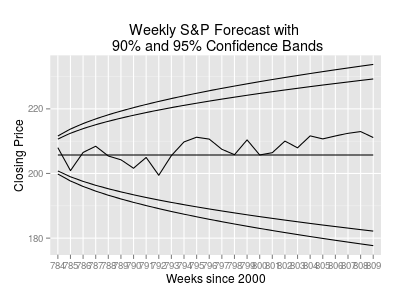
\includegraphics[scale=.4]{WeeklyNNPlot.png}
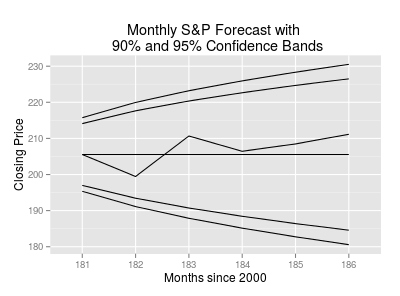
\includegraphics[scale=.4]{MonthlyNNPlot.png}
\end{center}

\end{frame}
%----------------------------------
% FRAME 7
%----------------------------------
\begin{frame}
\frametitle{}


\end{frame}

%----------------------------------------------------------------
% FRAME 8
%----------------------------------------------------------------

\begin{frame}
\frametitle{}

\end{frame}


%----------------------------------
% FRAME 9
%----------------------------------
\begin{frame}
	\frametitle{}

\end{frame}

%----------------------------------
% FRAME 10
%----------------------------------
\begin{frame}

	\frametitle{}

\end{frame}

%----------------------------------
% FRAME 11
%----------------------------------
\begin{frame}
	\frametitle{}

\end{frame}

%----------------------------------
% FRAME 12
%----------------------------------
\begin{frame}

\end{frame}

%----------------------------------
% FRAME 13
%----------------------------------
\begin{frame}
	\frametitle{}

\end{frame}

%----------------------------------
% FRAME 14
%----------------------------------

\begin{frame}
	\frametitle{}

\end{frame}

%----------------------------------
% FRAME 15
%----------------------------------

\begin{frame}
	\frametitle{Conclusions and Final Thoughts}
\end{frame}
\end{document}
